\documentclass{article}

\usepackage[margin=2.5cm]{geometry}

\usepackage[spanish]{babel}
\usepackage[T1]{fontenc}
\usepackage[utf8]{inputenc}


\usepackage{graphicx}
\usepackage{fancyhdr}
\usepackage{fancyvrb}

\usepackage{tcolorbox}

\usepackage{listings}
\usepackage{xcolor}

\definecolor{codegreen}{rgb}{.2,0.6,0}
\definecolor{codegray}{rgb}{0.5,0.5,0.5}
\definecolor{codepurple}{rgb}{0.58,0,0.82}
\definecolor{codeblue}{rgb}{0,0.4,0.82}
\definecolor{codeorange}{rgb}{0.94,0.34,0.0}
\definecolor{backcolour}{rgb}{0.95,0.95,0.92}
\definecolor{backcolourgray}{rgb}{0.92,0.92,0.92}
\definecolor{codewhite}{rgb}{1,1,1}

\lstdefinestyle{mystyle}{
    backgroundcolor=\color{backcolourgray},   
    commentstyle=\color{codegreen},
    keywordstyle=\color{codeblue},
    numberstyle=\tiny\color{black},
    stringstyle=\color{codeorange},
    basicstyle=\ttfamily\footnotesize,
    breakatwhitespace=false,         
    breaklines=true,                 
    captionpos=b,                    
    keepspaces=true,                 
    %numbers=left,                    
    numbersep=5pt,                  
    showspaces=false,                
    showstringspaces=false,
    showtabs=false,                  
    tabsize=2,
    extendedchars=true,
    frame=single
    %, basicstyle=\footnotesize
}
\lstset{style=mystyle}

\usepackage{hyperref}
\hypersetup{
    colorlinks=true,
    linkcolor=blue,
    filecolor=magenta,      
    urlcolor=cyan,
}

\pagestyle{fancy}
\fancyhf{}
\rhead{Sistemas Operativos. Práctica 3.}
\lhead{Pablo Cuesta Sierra y Álvaro Zamanillo Sáez}
\cfoot{\thepage}



\setlength{\parskip}{0.15cm}



\begin{document}

\title{Sistemas Operativos. Práctica 3.}
\author{Pablo Cuesta Sierra y Álvaro Zamanillo Sáez}
%\date{}
\maketitle

\begin{tcolorbox}
\tableofcontents
\end{tcolorbox}

\addcontentsline{toc}{subsection}{Pequeña nota sobre los ficheros}
\subsection*{Pequeña nota sobre los ficheros}

Al principio del desarrollo del proyecto, no sabíamos hasta que punto podíamos modificar los ficheros proporcionados, por lo que los tocamos lo mínimo e hicimos ficheros separados para el resto del código. En el fichero \emph{miner.h} únicamente hemos ampliado la estructura de la \emph{netdata} con algunos enteros y semáforos.

Nuestro proyecto está organizado de la siguiente forma:
\begin{itemize}
    \item
    Los \emph{main} de minero y monitor se encuentran, respectivamente, en \emph{mr\_miner.c} y \emph{mr\_monitor.c}.
    En este segundo fichero está, además, el código del hijo del monitor.
    
    \item
    \emph{mr\_util.h} contiene las declaraciones de las funciones comunes al proceso del minero y del monitor. Estas implementaciones están en \emph{mr\_util.c}.

    \item
    \emph{mr\_miner.h} contiene las declaraciones de las funciones del proceso del minero, implementadas en los ficheros \emph{mr\_miner\_func.c} y \emph{mr\_miner\_workers.c}

    \item 
    \emph{mr\_monitor.h} contiene las declaraciones de las funciones del proceso del mointor, implementadas en \emph{mr\_monitor\_func.c}.
\end{itemize}




\addcontentsline{toc}{subsection}{Sobre el número de trabajadores}
\subsection*{Sobre el número de trabajadores}

Como en el pdf del enunciado no se dice nada a cerca del número máximo de trabajadores, y a pesar de que en \emph{miner.h} hay una macro definida llamada \texttt{MAX\_WORKERS}, no hemos limitado el número de trabajadores. En el caso de que el número de trabajadores sea excesivo, de manera que no se pueda reservar la memoria o lanzar tantos hilos, el programa terminará liberando correctamente, tras mostrar el error por la terminal.



\addcontentsline{toc}{section}{Calificación base}
\section*{Calificación base}

\addcontentsline{toc}{subsection}{Nivel 1: Minero multihilo}
\subsection*{Nivel 1: Minero multihilo}

    Para este primer nivel hemos diferenciado dos partes. En primer lugar iniciar correctamente los segmentos de memoria compartida del bloque y la red, y por otro lado, la creación de los hilos y su correcta terminanción. 

    En la red, hemos incluido más atributos (para siguientes niveles) y es el primer minero el que se encarga de inicializarlos correctamente.
    De la misma forma, si el minero crea el segmento que corresponde al bloque, configura aleatoriamente una ``primera solución'', que se usará para generar el primer \textit{target} (y, por ende, el resto).

    Por otro lado, para lo relativo a los hilos, alocamos un \textit{array} de \texttt{pthread\_t} e iniciamos la estructura de minado que cada trabajador (hilo) va a recibir. Esta estructura solo se inicializa una vez pues es común para todas las rondas y se libera cuando el minero abandona la red. 
    
    \begin{lstlisting}[language=C, texcl=true]
        typedef struct Mine_struct_{
            long int target;
            long int begin; //índice por el que empieza a buscar el hilo
            long int end; //índice hasta el que el hilo busca (no incluido)
        } Mine_struct;  \end{lstlisting}


    En esta versión con un solo minero no se produce votación puesto que el \textit{quorum} siempre resulta en 1 minero activo. Por lo tanto, el minero siempre se considera ganador y añade el bloque minado a su propia cadena. La ronda de minado finaliza cuando un trabajdor encuentra la solución y manda una señal a su proceso para que salga de la función bloqueante \texttt{sigsuspend}. Todas las señales tratadas tienen el mismo manejador el cual solo pone a 1 la variable de tipo \texttt{sig\_atomic\_t} que indica que señal se ha recibido. Para distinguir si se sale de \texttt{sigsuspend} siendo ganador o perdedor, el trabajador que encuentra la solución manda a su proceso \texttt{SIGHUP} (el resto de mineros recibirán \texttt{SIGUSR2}).

    Los trabajadores de cada minero acaban cuando la variable \textit{end\_threads} vale 1. Esta variable se modifica cuando un hilo trabajador encuentra la solución o cuando el \textit{main} despierta tras recibir \texttt{SIGUSR2} de parte del ganador. El \textit{main} hace una llamada a \textit{pthread\_join} por cada hilo lanzado para asegurar que no hay pérdidas de memoria. La siguiente imagen muestra una ejecución de un minero con 1000 trabajdores y el análisis de Valgrind, mostrando que no hay pérdidas de memoria.

    \begin{figure}[h!]
        \centering
        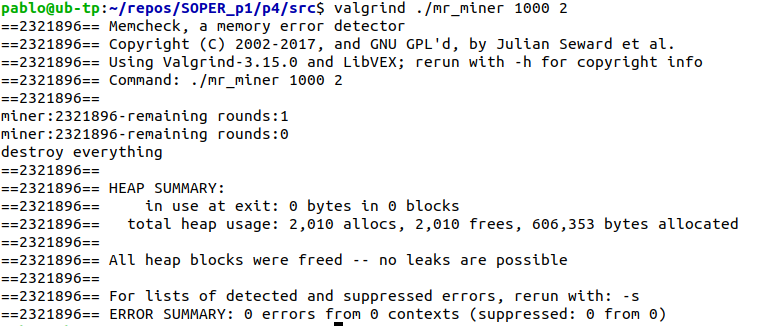
\includegraphics[scale=.41]{./pruebas/valgrind_1000_trabajadores}
        \caption{100 trabajadores con Valgrind}
    \end{figure}


    
    Al finalizar las rondas de minado se imprime la cadena de bloques en un fichero para lo cual hemos usado como base la función proporcionada cambiado \texttt{printf} por \texttt{dprintf}. Por último, el minero libera sus recursos con las respectivas funciones de \textit{free} y \textit{unlink}.

    

\addcontentsline{toc}{subsection}{Nivel 2: Comunicación con el monitor}
\subsection*{Nivel 2: Comunicación con el monitor}

    Para la comunciación con el monitor, se tiene que crear una cola de mensajes (a la que todos acceden abriéndola con su nombre). El primero en llegar la crea (sea minero o monitor), y los demás simplemente la abren.
    
    Además, el primero que llega, también crea los segmentos de memoria compartida e inicializa los campos a su respectivo valor inicial. Para evitar que dos procesos accedan a la vez en su escritura inicial, hemos tenido que usar un semáforo con nombre que impida el acceso simultáneo de dos procesos a la estructura compartida.
    Este \textit{mutex} es el único semáforo con nombre que hemos utilizado en el proyecto. Lo utilizamos para proteger escrituras simultáneas en los segmentos de memoria compartida.

    El único minero que hay por ahora, al declararse ganador, envía por la cola de mensajes su nuevo bloque.

    El monitor, como pone en los requisitos del enunciado, no comprueba que la solución sea la correcta (con la función \emph{hash}), sino que comprueba que si tiene un bloque con ese mismo \emph{id}, el bloque recibido tenga la misma solución y objetivo. Por este motivo, y como los mineros solo mandan los bloques que se han votado como correctos, no se da nunca el caso de que el monitor reconozca un ``bloque erróneo''.

    El monitor (proceso padre) le manda a su hijo los bloques nuevos. Para mandar el número de \emph{wallets} que el hijo imprime, hemos hecho uso del campo \texttt{is\_valid} del bloque que se escribe en la tubería, que no tiene ninguna utilidad en este caso, ya que el monitor solo recibe bloques válidos y, de todas formas, el hijo del monitor nunca utiliza este campo.
    
    Debido a que tanto el padre como el hijo pueden recibir señales durante la escritura o lectura en la \textit{pipe}, hemos utilizado el siguiente algoritmo, que asegura la lectura o escritura completa de la información y el manejo de las señales en cada caso (sería similar en el caso de la escritura, cambiando \emph{read} por \emph{write}):

    \begin{lstlisting}[language=C, texcl=true]
do
{
    size_read = read(fd[0], ((char*)block) + total_size_read, target_size - total_size_read);
    if (size_read == -1)
    {
        if(errno == EINTR && got_signal)
            handle_signal();
        else if(errno != EINTR)
            handle_read_error();
    }
    else if (size_read == 0)// se ha leído EOF
        return total_size_read;
    else
        total_size_read += size_read;
} while (total_size_read != target_size);\end{lstlisting}

    En el caso del hijo, \texttt{handle\_signal()} lo que hace es poner una nueva alarma de 5 segundos e imprimir toda la cadena en su fichero.

    En el caso del padre, cuando termina la lectura y ha recibido \texttt{SIGINT}, libera todo, cerrando la tubería y termina después de que su hijo haya finalizado.

    Al terminar, si el minero o el monitor ve que ya no hay más procesos enganchados a la memoria compartida, se encarga de borrar (\emph{unlink}) los segmentos de memoria compartida, el \emph{mutex} y la cola de mensajes.

\addcontentsline{toc}{subsubsection}{Problemas de saturación de la cola de mensajes}
\subsubsection*{Problemas de saturación de la cola de mensajes}

    Durante esta parte vimos un error que teóricamente podría ocurrir si el número de mineros activos fuese muy superior al tamaño de la cola de mensajes. En esta situación, si el monitor terminase mientras algunos procesos estuviesen bloqueados esperando a poder mandar el mensaje a la cola, estos mineros nunca saldrían de esa espera (a no ser que un nuevo monitor se lanzase). 
    
    
    %A pesar de que en las pruebas realizadas nunca hemos tenido este problema, gracias a los mecanismos de \textit{time out} (mencionados en el punto 5), este bloqueo se solucionaría ya que los mineros que sí lograron mandar un mensaje saldrían del bucle por una espera mayor a 3 segundos y ''arreglarían'' la red.
 

    Antes de implemantar los mecanismos de \textit{time out}, barajamos otras posibles soluciones pero las descartamos por los probelmas que acarreaban (uso de más señales) o por ser muy ineficientes. Estas son algunas de las ideas que descartamos:

    \begin{itemize}
        \item Opción 1: Antes de intentar mandar un mensaje, cada minero establece una alarma para evitar bloquearse más de un determinado número de segundos en la llamada \textit{mq\_send}.
        \item Opción 2: Aumentar el tamaño de la cola de mensajes. (teóricamente solo se evitaría el problema aumentándola al número máximo de mineros).
        \item Opción 3: Cuando un monitor finaliza, manda una señal a los mineros de la red para que los posibles mineros que estuviesen bloqueados en el envío del mensaje, se desbloqueen. 
    \end{itemize}



\addcontentsline{toc}{subsection}{Nivel 3: Red de mineros sin votación}
\subsection*{Nivel 3: Red de mineros sin votación}

En esta primera versión sin votación nuestro objetivo fue asegurar que los mineros empezasen las rondas a la vez, parasen de minar cuando otro minero hubiese encontrado la solución e impedir que dos mieros se declaren ganadores en una misma ronda. Los mineros que ingresan a la red deben esperar a que finalice la ronda actual, es decir, hasta que el ganador de la ronda les de paso a la siguiente ronda.

Tenemos que tener en cuenta que si el ganador de una ronda  va a salir (ya sea porque esta es su última ronda o porque ha recibido \texttt{SIGINT}), en la siguiente ronda la red debe seguir funcionando. Para esto, cada minero, si es su última ronda, `quita'\footnotemark su \textit{pid} (poniendo un valor negativo) del array de \textit{pids} y en caso de ser ganador, le cede el puesto al primer minero que encuentra (con \emph{pid} positivo).

\footnotetext{Esta medida de retirar su \emph{pid} es necesaria para que el minero que este haya declarado ganador no le devuelva la pelota a este en caso de que él también tenga que salirse en esta ronda.}

Para que esta medida sea efectiva, los mineros tienen que pararse al principio del bucle, hasta que todos los demás hayan terminado la anterior iteración (por si el ganador de la anterior ronda tiene que designar un ganador que prepare la ronda por él). Para esto, hemos puesto un mecanismo de \textit{turnstile}\footnotemark (cada minero, al principio del bucle, hace un \textit{down} y, seguidamente un \textit{up} del semáforo que hemos llamado \texttt{sem\_round\_end}). El semáforo está inicializado a 1 y el ganador de la ronda, antes de señalizar la finalización del recuento de votos, lo pone a 0 (con un \textit{down}) para `bloquear' la entrada
de mineros a la siguiente ronda. El último minero en finalizar la ronda hace \textit{up} del semáforo para permitir el paso a los demás.

\footnotetext{El término \textit{turnstile} proviene de \href{https://greenteapress.com/semaphores/LittleBookOfSemaphores.pdf}{The Little Book Of Semaphores}}

\addcontentsline{toc}{subsection}{Nivel 4: Red de mineros con votación}
\subsection*{Nivel 4: Red de mineros con votación}

En este nivel aseguramos  las siguientes restricciones de sincronización: los mineros perdedores no pueden empezar a votar hasta que el minero ganador haya subido la solución a memoria compartida y el minero ganador no puede empezar el recuento hasta que todos hayan votado.

Para la parte de la votación hemos usado dos semáforos. El primero \texttt{sem\_start\_voting} obliga a los perdedores a esperar a que el ganador haya preparado el bloque para la votación (subir la solución). Este semáforo anónimo (se encuentra en la memoria compartida de la red), es \textit{n-ario} y el ganador hace up tantas veces como votantes haya (número que ha sido calculado haciendo  recuento del \textit{quorum} anteriormente). Por otro lado, el ganador espera al semáforo \texttt{sem\_end\_votation} para hacer el recuento. Este semáforo solo toma valores 0 o 1, y es el último minero perdedor el que hace \emph{up} del semáforo tras votar. Finalmente, los perdedores han de esperar al resultado de la votación. Esta condición de sincronización se resuelve igual que la de esperar para comenzar a votar; en este caso usamos el semáforo \texttt{sem\_scrutiny}.

En general la idea usada para resolver la sincronización de la votación es reducirlo al caso de dos procesos: un proceso ganador y un proceso perdedor (salvo que este proceso es en realidad un grupo de procesos). De esta forma se trata de un problema de \textit{leader \& follower}. Los semáforos del ganador toman valores 0 o 1, mientras que los del grupo perdedor, son semáforos que toman valores (posiblemente) de 0 a $n$. Asimismo, el modelo usado para que el último votante avise al ganador ha sido \textit{lightswitchoff}.

\subsubsection*{Probando la votación}
Con el código implementado si un minero se declara ganador es porque verdaderamente ha encontrado una solución. Es por eso que las votaciones siempre tenían el mismo resultado: ningún voto en contra. Para probar de forma muy simple lo implementado hicimos que el  \textit{simple\_hash()} dependiese de la paridad del \textit{PID} del minero, de forma que un minero con \textit{PID} par votase siempre en contra de una solución encontrada por un minero con \textit{PID} impar y viceversa. Con este cambio rápido pudimos probar (de una forma muy limitada) votaciones que no siempre resultasen favorables.


\addcontentsline{toc}{subsection}{Nivel 5}
\subsection*{Nivel 5}

El último requisito que nos faltaba era poner una espera con tiempo máximo en los semáforos, que tenemos ahora para que si un minero se queda pillado en algún punto o termina inesperadamente, el resto deje de esperar y termine. Para esto, hemos usado \texttt{sem\_timedwait}. 

Aunque improbable, se podría dar que un fuese  extremadamente lento en comparación con el resto (por ejemplo, ejecutando un minero con \textit{valgrind}). Cuando el resto de mineros se percataban de esto y terminaban su ejecución, muchas veces los semáforos quedaban con valores incorrectos que impedían el correcto funcionamiento de la red. Para evitar esto, usamos una variable en la memoria compartida que cuenta el número de mineros activos, de modo que si un minero va a liberar y se da cuenta de que es el último minero activo, destruye todos los semáforos, para que el primer minero que llegue los inicialice correctamente evitando así posibles problemas.

\addcontentsline{toc}{section}{Mejoras}
\section*{Mejoras}

\addcontentsline{toc}{subsection}{Un único monitor activo}
\subsection*{Un único monitor activo}
La primera mejora introducida es impedir que haya dos monitores activos. Si la red cuenta con un monitor y se intenta lanzar otro, este segundo proceso finalizará. La implementación de esta mejora se reduce a un bloque \emph{if} en la función que inicia el segmento de memoria compartida del monitor.

\addcontentsline{toc}{subsection}{Mantenimiento de la red en caso de la salida repentina de un minero ganador}
\subsection*{Mantenimiento de la red en caso de la salida repentina de un ganador}
La siguiente mejora extiende el requisito de la práctica de que si el minero ganador de un ronda sufre un problema y no prepara la siguiente ronda, el resto de mineros puede terminar. En nuestro caso si el ganador de la última ronda recibe \texttt{SIGINT} (y, por lo tanto, debe finalizar), ``asignará el título de último ganador'' a un minero activo (como ya se ha explicado en el Nivel 3). Para asegurarnos de que la red continúe funcionando incluso si un minero recibe \texttt{SIGINT}, debemos permitir que se reciba esta señal antes de comprobar si esta ronda es la última del minero. Para ello, en el bucle de las rondas, quitamos y volvemos a poner la máscara del proceso (con \texttt{sigprocmask}). 

\subsubsection*{Muerte de un minero de forma repentina}
Siguiendo con el buen funcionamiento de la red cuando un minero muere, hemos implementado que la red pueda recuperarse de la muerte de un minero de forma no controlada, como, por ejemplo, al recibir \texttt{SIGKILL}. Cuando un minero muere durante una ronda, el resto de mineros finalizaran debido a los mecanismos de \textit{time out} implementados; no obstante, quedaba la cuestión de liberar correctamente los recursos o resetear los parámetros correspondientes por si se lanzaban más mineros. Lo que hacemos es que el primer minero que salga del bucle por un \textit{time out}, ajustará el número de mineros (que será superior al verdadero ya que los que han muerto de forma descontrolada no notificaron su baja) de forma que el último minero en acabar libere todo. De esta forma conseguimos que cuando se manda \texttt{SIGKILL} a un minero, el resto de mineros se ven forzados a terminar pero los mineros que se lancen a continuación (si la red se mantiene activa por la presencia de un monitor) podrán volver a minar con normalidad.


\end{document}

por quitar::
    
    makefile

    destroy everything
